\section{Exploratory Data Analysis}

One simple yet useful way to explore a data-set is to visualize the feature distribution for each class.
In our situation this is simply not possible and not very insightful as we have too many features.
To be precise 728 = $28\times28$ features/pixels.
This doesn't mean the data-set can't be visualized, which we will discuss in the next section.

\subsection{Principal Component Analysis}\label{subsec:principal-component-analysis}
As mentioned before due to our large data-set it is hard to visualize feature distributions, this is where principal component analysis or PCA can be used instead.
Principal Component Analysis (PCA) is a dimensionality reduction technique used to reduce the number of features in a dataset, while still preserving the most important information.
It does this by transforming variables into a new set of variables, called principal components, which are uncorrelated from each other and explain the maximum amount of variance in the data.
Below we explore the relationships between the first 3 principal components.
These 3 principal components represent the direction of most variance in the original data\\
\begin{figure}[ht]
    \centering
    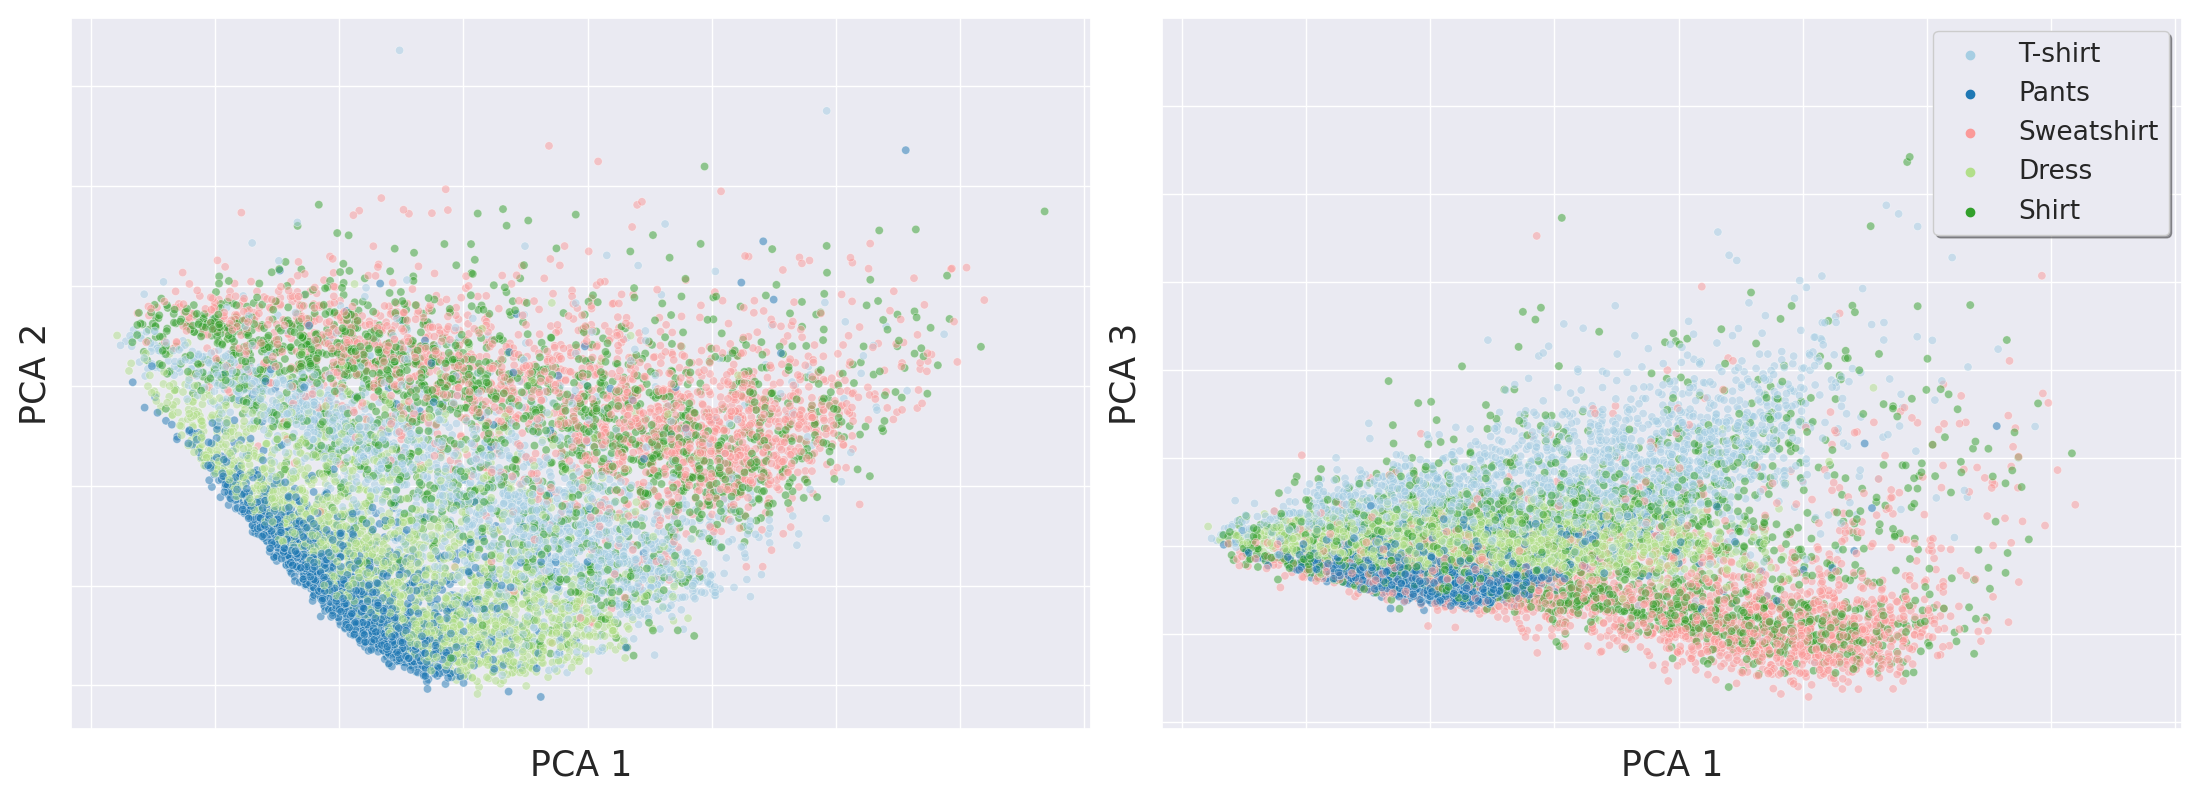
\includegraphics[scale=0.32]{figures_for_report/PCA}
    \captionsetup{justification=centering,margin=2cm}
    \caption{Visualizing relationships between first 3 PCA's}\label{fig:figure}
\end{figure}

